% Created 2021-12-22 Wed 12:26
% Intended LaTeX compiler: pdflatex
\documentclass[12pt]{article}

%%%% settings when exporting code %%%% 

\usepackage{listings}
\lstdefinestyle{code-small}{
backgroundcolor=\color{white}, % background color for the code block
basicstyle=\ttfamily\small, % font used to display the code
commentstyle=\color[rgb]{0.5,0,0.5}, % color used to display comments in the code
keywordstyle=\color{black}, % color used to highlight certain words in the code
numberstyle=\ttfamily\tiny\color{gray}, % color used to display the line numbers
rulecolor=\color{black}, % color of the frame
stringstyle=\color[rgb]{0,.5,0},  % color used to display strings in the code
breakatwhitespace=false, % sets if automatic breaks should only happen at whitespace
breaklines=true, % sets automatic line breaking
columns=fullflexible,
frame=single, % adds a frame around the code (non,leftline,topline,bottomline,lines,single,shadowbox)
keepspaces=true, % % keeps spaces in text, useful for keeping indentation of code
literate={~}{$\sim$}{1}, % symbol properly display via latex
numbers=none, % where to put the line-numbers; possible values are (none, left, right)
numbersep=10pt, % how far the line-numbers are from the code
showspaces=false,
showstringspaces=false,
stepnumber=1, % the step between two line-numbers. If it's 1, each line will be numbered
tabsize=1,
xleftmargin=0cm,
emph={anova,apply,class,coef,colnames,colNames,colSums,dim,dcast,for,ggplot,head,if,ifelse,is.na,lapply,list.files,library,logLik,melt,plot,require,rowSums,sapply,setcolorder,setkey,str,summary,tapply},
aboveskip = \medskipamount, % define the space above displayed listings.
belowskip = \medskipamount, % define the space above displayed listings.
lineskip = 0pt} % specifies additional space between lines in listings
\lstset{style=code-small}
%%%% packages %%%%%

\usepackage[utf8]{inputenc}
\usepackage[T1]{fontenc}
\usepackage{lmodern}
\usepackage{textcomp}
\usepackage{color}
\usepackage{graphicx}
\usepackage{grffile}
\usepackage{wrapfig}
\usepackage{rotating}
\usepackage{longtable}
\usepackage{multirow}
\usepackage{multicol}
\usepackage{changes}
\usepackage{pdflscape}
\usepackage{geometry}
\usepackage[normalem]{ulem}
\usepackage{amssymb}
\usepackage{amsmath}
\usepackage{amsfonts}
\usepackage{dsfont}
\usepackage{array}
\usepackage{ifthen}
\usepackage{hyperref}
\usepackage{natbib}
\RequirePackage{setspace} % to modify the space between lines - incompatible with footnote in beamer
\renewcommand{\baselinestretch}{1.1}
\geometry{a4paper, left=10mm, right=10mm, top=10mm}
\usepackage{titlesec}
\usepackage{etoolbox}

\makeatletter
\patchcmd{\ttlh@hang}{\parindent\z@}{\parindent\z@\leavevmode}{}{}
\patchcmd{\ttlh@hang}{\noindent}{}{}{}
\makeatother
\RequirePackage{colortbl} % arrayrulecolor to mix colors
\definecolor{myorange}{rgb}{1,0.2,0}
\definecolor{mypurple}{rgb}{0.7,0,8}
\definecolor{mycyan}{rgb}{0,0.6,0.6}
\newcommand{\lightblue}{blue!50!white}
\newcommand{\darkblue}{blue!80!black}
\newcommand{\darkgreen}{green!50!black}
\newcommand{\darkred}{red!50!black}
\definecolor{gray}{gray}{0.5}
\hypersetup{
citecolor=[rgb]{0,0.5,0},
urlcolor=[rgb]{0,0,0.5},
linkcolor=[rgb]{0,0,0.5},
}
\newenvironment{note}{\small \color{gray}\fontfamily{lmtt}\selectfont}{\par}
\newenvironment{activity}{\color{orange}\fontfamily{qzc}\selectfont}{\par}
\RequirePackage{pifont}
\RequirePackage{relsize}
\newcommand{\Cross}{{\raisebox{-0.5ex}%
{\relsize{1.5}\ding{56}}}\hspace{1pt} }
\newcommand{\Valid}{{\raisebox{-0.5ex}%
{\relsize{1.5}\ding{52}}}\hspace{1pt} }
\newcommand{\CrossR}{ \textcolor{red}{\Cross} }
\newcommand{\ValidV}{ \textcolor{green}{\Valid} }
\usepackage{stackengine}
\usepackage{scalerel}
\newcommand\Warning[1][3ex]{%
\renewcommand\stacktype{L}%
\scaleto{\stackon[1.3pt]{\color{red}$\triangle$}{\tiny\bfseries !}}{#1}%
\xspace
}
\newcommand\Rlogo{\textbf{\textsf{R}}\xspace} %
\RequirePackage{fancyvrb}
\DefineVerbatimEnvironment{verbatim}{Verbatim}{fontsize=\small,formatcom = {\color[rgb]{0.5,0,0}}}
\RequirePackage{enumitem} % better than enumerate
\RequirePackage{epstopdf} % to be able to convert .eps to .pdf image files
\RequirePackage{capt-of} %
\RequirePackage{caption} % newlines in graphics
\RequirePackage{tikz-cd} % graph
\RequirePackage{booktabs} % for nice lines in table (e.g. toprule, bottomrule, midrule, cmidrule)
\RequirePackage{amsmath}
\RequirePackage{algorithm}
\RequirePackage[noend]{algpseudocode}
\RequirePackage{dsfont}
\RequirePackage{amsmath,stmaryrd,graphicx}
\RequirePackage{prodint} % product integral symbol (\PRODI)
\usepackage{ifthen}
\usepackage{xifthen}
\usepackage{xargs}
\usepackage{xspace}
\newcommand\defOperator[7]{%
\ifthenelse{\isempty{#2}}{
\ifthenelse{\isempty{#1}}{#7{#3}#4}{#7{#3}#4 \left#5 #1 \right#6}
}{
\ifthenelse{\isempty{#1}}{#7{#3}#4_{#2}}{#7{#3}#4_{#1}\left#5 #2 \right#6}
}
}
\newcommand\defUOperator[5]{%
\ifthenelse{\isempty{#1}}{
#5\left#3 #2 \right#4
}{
\ifthenelse{\isempty{#2}}{\underset{#1}{\operatornamewithlimits{#5}}}{
\underset{#1}{\operatornamewithlimits{#5}}\left#3 #2 \right#4}
}
}
\newcommand{\defBoldVar}[2]{
\ifthenelse{\equal{#2}{T}}{\boldsymbol{#1}}{\mathbf{#1}}
}
\newcommandx\Esp[2][1=,2=]{\defOperator{#1}{#2}{E}{}{\lbrack}{\rbrack}{\mathbb}}
\newcommandx\Prob[2][1=,2=]{\defOperator{#1}{#2}{P}{}{\lbrack}{\rbrack}{\mathbb}}
\newcommandx\Qrob[2][1=,2=]{\defOperator{#1}{#2}{Q}{}{\lbrack}{\rbrack}{\mathbb}}
\newcommandx\Var[2][1=,2=]{\defOperator{#1}{#2}{V}{ar}{\lbrack}{\rbrack}{\mathbb}}
\newcommandx\Cov[2][1=,2=]{\defOperator{#1}{#2}{C}{ov}{\lbrack}{\rbrack}{\mathbb}}
\newcommandx\Binom[2][1=,2=]{\defOperator{#1}{#2}{B}{}{(}{)}{\mathcal}}
\newcommandx\Gaus[2][1=,2=]{\defOperator{#1}{#2}{N}{}{(}{)}{\mathcal}}
\newcommandx\Wishart[2][1=,2=]{\defOperator{#1}{#2}{W}{ishart}{(}{)}{\mathcal}}
\newcommandx\Likelihood[2][1=,2=]{\defOperator{#1}{#2}{L}{}{(}{)}{\mathcal}}
\newcommandx\logLikelihood[2][1=,2=]{\defOperator{#1}{#2}{\ell}{}{(}{)}{}}
\newcommandx\Information[2][1=,2=]{\defOperator{#1}{#2}{I}{}{(}{)}{\mathcal}}
\newcommandx\Score[2][1=,2=]{\defOperator{#1}{#2}{S}{}{(}{)}{\mathcal}}
\newcommandx\Vois[2][1=,2=]{\defOperator{#1}{#2}{V}{}{(}{)}{\mathcal}}
\newcommandx\IF[2][1=,2=]{\defOperator{#1}{#2}{IF}{}{(}{)}{\mathcal}}
\newcommandx\Ind[1][1=]{\defOperator{}{#1}{1}{}{(}{)}{\mathds}}
\newcommandx\Max[2][1=,2=]{\defUOperator{#1}{#2}{(}{)}{min}}
\newcommandx\Min[2][1=,2=]{\defUOperator{#1}{#2}{(}{)}{max}}
\newcommandx\argMax[2][1=,2=]{\defUOperator{#1}{#2}{(}{)}{argmax}}
\newcommandx\argMin[2][1=,2=]{\defUOperator{#1}{#2}{(}{)}{argmin}}
\newcommandx\cvD[2][1=D,2=n \rightarrow \infty]{\xrightarrow[#2]{#1}}
\newcommandx\Hypothesis[2][1=,2=]{
\ifthenelse{\isempty{#1}}{
\mathcal{H}
}{
\ifthenelse{\isempty{#2}}{
\mathcal{H}_{#1}
}{
\mathcal{H}^{(#2)}_{#1}
}
}
}
\newcommandx\dpartial[4][1=,2=,3=,4=\partial]{
\ifthenelse{\isempty{#3}}{
\frac{#4 #1}{#4 #2}
}{
\left.\frac{#4 #1}{#4 #2}\right\rvert_{#3}
}
}
\newcommandx\dTpartial[3][1=,2=,3=]{\dpartial[#1][#2][#3][d]}
\newcommandx\ddpartial[3][1=,2=,3=]{
\ifthenelse{\isempty{#3}}{
\frac{\partial^{2} #1}{\partial #2^2}
}{
\frac{\partial^2 #1}{\partial #2\partial #3}
}
}
\newcommand\Real{\mathbb{R}}
\newcommand\Rational{\mathbb{Q}}
\newcommand\Natural{\mathbb{N}}
\newcommand\trans[1]{{#1}^\intercal}%\newcommand\trans[1]{{\vphantom{#1}}^\top{#1}}
\newcommand{\independent}{\mathrel{\text{\scalebox{1.5}{$\perp\mkern-10mu\perp$}}}}
\newcommand\half{\frac{1}{2}}
\newcommand\normMax[1]{\left|\left|#1\right|\right|_{max}}
\newcommand\normTwo[1]{\left|\left|#1\right|\right|_{2}}
\newcommand\Veta{\boldsymbol{\eta}}
\newcommand\VX{\mathbf{X}}
\author{Brice Ozenne}
\date{\today}
\title{Overview of the package BuyseTest}
\hypersetup{
 colorlinks=true,
 pdfauthor={Brice Ozenne},
 pdftitle={Overview of the package BuyseTest},
 pdfkeywords={},
 pdfsubject={},
 pdfcreator={Emacs 26.3 (Org mode 9.4.6)},
 pdflang={English}
 }
\begin{document}

\maketitle
This vignette describes the main functionalities of the \textbf{BuyseTest}
package. This package implements the Generalized Pairwise Comparisons
(GPC) as defined in \cite{buyse2010generalized} for complete
observations, and extended in \cite{peron2018extension} to deal with
right-censoring. When considering a single endpoint, the GPC procedure
can be summarized as follow. Denote the endpoint by \(Y\) in the
treatment group and by \(X\) in the control group. Given a threshold
of clinical relevance \(\tau\), the aim of GPC is to estimate the
proportion in favor of treatment \(\Prob[Y \geq X + \tau]\) and the
proportion in favor of control \(\Prob[X \geq Y + \tau]\). Other
statistics such as the net benefit \(\Prob[Y \geq X + \tau]-\Prob[X
\geq Y + \tau]\) or the win ratio \(\frac{\Prob[Y \geq X +
\tau]}{\Prob[X \geq Y + \tau]}\) can then be deduced. The vignette is
written for readers familar with the GPC framework \footnote{if not,
\cite{buyse2010generalized} is a good place to start.}, e.g. prioritized
endpoints, pair, net benefit, win ratio, threshold of clinical
relevance, \ldots, since it focuses on the software aspect
of the \textbf{BuyseTest} package (not on the underlying statistical model).

\bigskip

The \textbf{BuyseTest} package contains three main functions:
\begin{itemize}
\item the function \texttt{BuyseTest} is the main function of the package. It
performs the GPC, estimates the net benefit/win ratio, and output a
\emph{BuyseRes} object. The user can interact with \emph{BuyseRes} objects using:
\begin{itemize}
\item \texttt{summary} to obtain a nice display of the results
\item \texttt{coef} to extract the estimates.
\item \texttt{confint} to extract estimates, confidence intervals, and p.values.
\item \texttt{sensitivity} to perform a sensitivity analysis on the choice of the threshold(s) of clinical relevance.
\item \texttt{getIid} to extract the iid decomposition of the estimator.
\item \texttt{getPairScore} to extract the contribution of each pair to the net benefit/win ratio.
\item \texttt{getSurvival} to extract the estimates of the survival (only relevant for right-censored endpoints).
\end{itemize}
\item the \texttt{powerBuyseTest} function performs simulation studies,
e.g. to estimate the statistical power or assess the bias / type 1
error rate of a test for a specific design.
\item the \texttt{BuyseTest.options} function enables the user to display the
default values used in the \textbf{BuyseTest} package (essentially used by
the \texttt{BuyseTest} function). function. The function can also change
the default values to better match the user needs.
\end{itemize}

\clearpage

Before going further we need to load the \textbf{BuyseTest} package in the R
session:
\lstset{language=r,label= ,caption= ,captionpos=b,numbers=none}
\begin{lstlisting}
library(BuyseTest)
library(data.table)
\end{lstlisting}

To illustrate the functionalities of the package, we will used the
\texttt{veteran} dataset from the \textbf{survival} package:
\lstset{language=r,label= ,caption= ,captionpos=b,numbers=none}
\begin{lstlisting}
library(survival)
head(veteran)
\end{lstlisting}

\begin{verbatim}
  trt celltype time status karno diagtime age prior
1   1 squamous   72      1    60        7  69     0
2   1 squamous  411      1    70        5  64    10
3   1 squamous  228      1    60        3  38     0
4   1 squamous  126      1    60        9  63    10
5   1 squamous  118      1    70       11  65    10
6   1 squamous   10      1    20        5  49     0
\end{verbatim}


See \texttt{?veteran} for a presentation of the database.

\bigskip

\uline{Note:} the \textbf{BuyseTest} package is under active development. Newer
package versions may include additional functionalities and fix
previous bugs. The version of the package that is being is:
\lstset{language=r,label= ,caption= ,captionpos=b,numbers=none}
\begin{lstlisting}
utils::packageVersion("BuyseTest")
\end{lstlisting}

\begin{verbatim}
[1] ‘2.3.9’
\end{verbatim}


For completness, the details of the R session used to generate this
document are:
\lstset{language=r,label= ,caption= ,captionpos=b,numbers=none}
\begin{lstlisting}
sessionInfo()
\end{lstlisting}

\begin{verbatim}
R version 4.1.2 (2021-11-01)
Platform: x86_64-pc-linux-gnu (64-bit)
Running under: Ubuntu 20.04.3 LTS

Matrix products: default
BLAS:   /usr/lib/x86_64-linux-gnu/blas/libblas.so.3.9.0
LAPACK: /usr/lib/x86_64-linux-gnu/lapack/liblapack.so.3.9.0

locale:
 [1] LC_CTYPE=en_US.UTF-8       LC_NUMERIC=C               LC_TIME=en_US.UTF-8       
 [4] LC_COLLATE=en_US.UTF-8     LC_MONETARY=en_US.UTF-8    LC_MESSAGES=en_US.UTF-8   
 [7] LC_PAPER=en_US.UTF-8       LC_NAME=C                  LC_ADDRESS=C              
[10] LC_TELEPHONE=C             LC_MEASUREMENT=en_US.UTF-8 LC_IDENTIFICATION=C       

attached base packages:
[1] stats     graphics  grDevices utils     datasets  methods   base     

other attached packages:
[1] data.table_1.14.0  BuyseTest_2.3.9    Rcpp_1.0.7         prodlim_2019.11.13
[5] ggplot2_3.3.5      survival_3.2-13   

loaded via a namespace (and not attached):
 [1] pillar_1.6.4       compiler_4.1.2     tools_4.1.2        digest_0.6.28     
 [5] lifecycle_1.0.1    tibble_3.1.5       gtable_0.3.0       lattice_0.20-45   
 [9] pkgconfig_2.0.3    rlang_0.4.12       Matrix_1.4-0       DBI_1.1.1         
[13] parallel_4.1.2     SparseM_1.81       withr_2.4.2        dplyr_1.0.7       
[17] MatrixModels_0.5-0 generics_0.1.0     vctrs_0.3.8        globals_0.14.0    
[21] stats4_4.1.2       grid_4.1.2         tidyselect_1.1.1   glue_1.4.2        
[25] listenv_0.8.0      R6_2.5.1           future.apply_1.8.1 fansi_0.5.0       
[29] parallelly_1.28.1  lava_1.6.10        purrr_0.3.4        magrittr_2.0.1    
[33] scales_1.1.1       codetools_0.2-18   ellipsis_0.3.2     splines_4.1.2     
[37] assertthat_0.2.1   future_1.23.0      colorspace_2.0-2   utf8_1.2.2        
[41] munsell_0.5.0      crayon_1.4.2
\end{verbatim}

\clearpage

\section{Performing generalized pairwise comparisons (GPC) using the \texttt{BuyseTest} function}
\label{sec:orga0e93a1}

To perform generalized pairwise comparisons, the \texttt{BuyseTest} function needs:
\begin{itemize}
\item where the data are stored \hfill - argument \texttt{data}
\item the name of the endpoints \hfill - argument \texttt{endpoint}
\item the type of each endpoint \hfill - argument \texttt{type}
\item the variable defining the two treatment groups \hfill - argument
\texttt{treatment}
\end{itemize}
The \texttt{BuyseTest} function has many optional arguments to specify for example:
\begin{itemize}
\item the threshold of clinical relevance associated to each endpoint \hfill - argument \texttt{threshold}
\item the censoring associated to each endpoint (for time to event endpoints) \hfill - argument \texttt{status}
\end{itemize}

\bigskip

There are two equivalent ways to define the GPC: 
\begin{itemize}
\item using a separate argument for each element:
\end{itemize}

\lstset{language=r,label= ,caption= ,captionpos=b,numbers=none}
\begin{lstlisting}
BT <- BuyseTest(data = veteran, 
		endpoint = "time", 
		type = "timeToEvent", 
		treatment = "trt", 
		status = "status", 
		threshold = 20)
\end{lstlisting}

\begin{verbatim}

         Generalized Pairwise Comparisons

Settings 
   - 2 groups  : Control = 1 and Treatment = 2
   - 1 endpoint: 
       priority endpoint type           operator             threshold event       
       1        time     time to event  higher is favorable  20        status (0 1)
   - right-censored pairs: probabilistic score based on the survival curves 

Point estimation and calculation of the iid decomposition

Estimation of the estimator's distribution 
   - method: moments of the U-statistic

Gather the results in a S4BuyseTest object
\end{verbatim}

\clearpage

\begin{itemize}
\item or via a formula interface. In the formula interface endpoint are
wrapped by parentheses. The parentheses must be preceded by their
type: 
\begin{itemize}[label={-}]
\item binary (\texttt{b}, \texttt{bin}, or \texttt{binary})
\item continuous (\texttt{c}, \texttt{cont}, or  \texttt{continuous})
\item time to event (\texttt{t}, \texttt{tte}, or \texttt{timetoevent})
\end{itemize}
\end{itemize}

\lstset{language=r,label= ,caption= ,captionpos=b,numbers=none}
\begin{lstlisting}
BT.f <- BuyseTest(trt ~ tte(time, threshold = 20, status = "status"),
		  data = veteran)
\end{lstlisting}

\begin{verbatim}

         Generalized Pairwise Comparisons

Settings 
   - 2 groups  : Control = 1 and Treatment = 2
   - 1 endpoint: 
       priority endpoint type           operator             threshold event       
       1        time     time to event  higher is favorable  20        status (0 1)
   - right-censored pairs: probabilistic score based on the survival curves 

Point estimation and calculation of the iid decomposition

Estimation of the estimator's distribution 
   - method: moments of the U-statistic

Gather the results in a S4BuyseTest object
\end{verbatim}

We can check that the two approaches are equivalent:
\lstset{language=r,label= ,caption= ,captionpos=b,numbers=none}
\begin{lstlisting}
BT.f@call <- list(); BT@call <- list();
testthat::expect_equal(BT.f,BT)
\end{lstlisting}

\subsection{Displaying the results}
\label{sec:orgea24ddf}

The results of the GPC can be displayed using the \texttt{summary} method:
\lstset{language=r,label= ,caption= ,captionpos=b,numbers=none}
\begin{lstlisting}
summary(BT)
\end{lstlisting}

\begin{verbatim}
      Generalized pairwise comparisons with 1 endpoint

- statistic       : net benefit (delta: endpoint specific, Delta: global) 
- null hypothesis : Delta == 0 
- confidence level: 0.95 
- inference       : H-projection of order 1
- treatment groups: 2 (treatment) vs. 1 (control) 
- censored pairs  : probabilistic score based on the survival curves
- results
endpoint threshold total(%) favorable(%) unfavorable(%) neutral(%) uninf(%)   Delta
    time        20      100        37.78          46.54      15.68        0 -0.0877
CI [2.5% ; 97.5%] p.value 
 [-0.2735;0.1045] 0.37162
\end{verbatim}

 To display the number of pairs instead of the percentage of pairs
that are favorable/unfavorable/neutral/uniformative, set the argument
\texttt{percentage} to \texttt{FALSE}:
\lstset{language=r,label= ,caption= ,captionpos=b,numbers=none}
\begin{lstlisting}
summary(BT, percentage = FALSE)
\end{lstlisting}

\begin{verbatim}
      Generalized pairwise comparisons with 1 endpoint

- statistic       : net benefit (delta: endpoint specific, Delta: global) 
- null hypothesis : Delta == 0 
- confidence level: 0.95 
- inference       : H-projection of order 1
- treatment groups: 2 (treatment) vs. 1 (control) 
- censored pairs  : probabilistic score based on the survival curves
- results
endpoint threshold total favorable unfavorable neutral uninf   Delta CI [2.5% ; 97.5%]
    time        20  4692   1772.59     2183.89  735.52     0 -0.0877  [-0.2735;0.1045]
p.value 
0.37162
\end{verbatim}

\bigskip

By default \texttt{summary} displays results relative to the net benefit. To
get results for the win ratio set the argument \texttt{statistic} to
"winRatio":
\lstset{language=r,label= ,caption= ,captionpos=b,numbers=none}
\begin{lstlisting}
summary(BT, statistic = "winRatio")
\end{lstlisting}

\begin{verbatim}
      Generalized pairwise comparisons with 1 endpoint

- statistic       : win ratio (delta: endpoint specific, Delta: global) 
- null hypothesis : Delta == 1 
- confidence level: 0.95 
- inference       : H-projection of order 1
- treatment groups: 2 (treatment) vs. 1 (control) 
- censored pairs  : probabilistic score based on the survival curves
- results
endpoint threshold total(%) favorable(%) unfavorable(%) neutral(%) uninf(%)  Delta
    time        20      100        37.78          46.54      15.68        0 0.8117
CI [2.5% ; 97.5%] p.value 
  [0.5134;1.2833] 0.37195
\end{verbatim}

See \texttt{help(BuyseRes-summary)} for more detailed explanations about the
\texttt{summary} method and its output. Note that a more concise output, in a
data.frame format, can be obtained via the \texttt{confint} method:
\lstset{language=r,label= ,caption= ,captionpos=b,numbers=none}
\begin{lstlisting}
confint(BT, statistic = "winRatio")
\end{lstlisting}

\begin{verbatim}
          estimate        se  lower.ci upper.ci null   p.value
time_t20 0.8116692 0.1896937 0.5133887 1.283252    1 0.3719466
\end{verbatim}

\subsection{Stratified GPC}
\label{sec:orgfbcebe7}

GPC can be performed for subgroups of a categorical variable \hfill -
argument \texttt{strata}

\bigskip

 For instance, the celltype may have huge influence on the survival
time and the investigator would like to only compare patients that
have the same celltype. In the formula interface this is achieved by
adding a single variable in the right hand side of the formula:
\lstset{language=r,label= ,caption= ,captionpos=b,numbers=none}
\begin{lstlisting}
ffstrata <- trt ~ tte(time, threshold = 20, status = "status") + celltype
BTstrata <- BuyseTest(ffstrata, data = veteran, trace = 0)
\end{lstlisting}

Not being wrapped by \texttt{bin}, \texttt{cont} or \texttt{tte} differentiates it from
endpoint variables.

\bigskip

When doing a stratified analysis, the summary method displays the
global results as well as the results within each strata\footnote{the
strata-specific results can be removed by setting the argument
\texttt{strata} to \texttt{"global"} when calling \texttt{summary}.}:
\lstset{language=r,label= ,caption= ,captionpos=b,numbers=none}
\begin{lstlisting}
summary(BTstrata, type.display = c("endpoint","threshold","strata",
			      "total","favorable","unfavorable","delta","Delta"))
\end{lstlisting}

\begin{verbatim}
      Generalized pairwise comparisons with 1 endpoint and 4 strata

- statistic       : net benefit (delta: endpoint specific, Delta: global) 
- null hypothesis : Delta == 0 
- confidence level: 0.95 
- inference       : H-projection of order 1
- treatment groups: 2 (treatment) vs. 1 (control) 
- censored pairs  : probabilistic score based on the survival curves
- uninformative pairs: no contribution
- results
endpoint threshold    strata total(%) favorable(%) unfavorable(%)   Delta
    time        20    global   100.00        36.06          45.77 -0.0971
                    squamous    25.38        14.33           8.77        
                   smallcell    45.69        12.69          20.88        
                       adeno    13.71         4.74           6.15        
                       large    15.23         4.30           9.97
\end{verbatim}

Note that here the numbers in the total/favorable/unfavorable/ columns
are relative to the overall sample while the delta is only relative to
the strata. The global delta is a sum of the strata specific delta
weighted by the empirical proportion of pairs for each strata.

\clearpage

\subsection{Using multiple endpoints}
\label{sec:orgd3c8ed5}
More than one endpoint can be considered by indicating a vector of
endpoints, types, and thresholds. In the formula interface, the
different endpoints must be separated with a "+" on the right hand
side of the formula:
\lstset{language=r,label= ,caption= ,captionpos=b,numbers=none}
\begin{lstlisting}
ff2 <- trt ~ tte(time, threshold = 20, status = "status") + cont(karno, threshold = 0)
BT.H <- BuyseTest(ff2, data = veteran, trace = 0)
summary(BT.H)
\end{lstlisting}

\begin{verbatim}
      Generalized pairwise comparisons with 2 prioritized endpoints

- statistic       : net benefit (delta: endpoint specific, Delta: global) 
- null hypothesis : Delta == 0 
- confidence level: 0.95 
- inference       : H-projection of order 1
- treatment groups: 2 (treatment) vs. 1 (control) 
- censored pairs  : probabilistic score based on the survival curves
- neutral pairs   : re-analyzed using lower priority endpoints
- results
endpoint threshold total(%) favorable(%) unfavorable(%) neutral(%) uninf(%)   delta   Delta
    time        20   100.00        37.78          46.54      15.68        0 -0.0877 -0.0877
   karno              15.68         5.78           7.11       2.78        0 -0.0133 -0.1009
CI [2.5% ; 97.5%] p.value 
 [-0.2735;0.1045] 0.37162 
 [-0.2901;0.0959] 0.31478
\end{verbatim}

The hierarchy of the endpoint is defined from left (most important
endpoint, here \texttt{time}) to right (least important endpoint, here
\texttt{karno}). In the \texttt{summary} output, the confidence intervals and
p.values are computed for the column \texttt{Delta}, i.e. here the net
benefit for the first endpoint (line 1) and the the first and second
endpoint (line 2). In other words, the last confidence interval and
p-value is the one for the analysis over all endpoints (generally the
one to report).

\bigskip

It is also possible to perform the comparisons on all pairs for all
endpoints by setting the argument \texttt{hierarchical} to \texttt{FALSE}:
\lstset{language=r,label= ,caption= ,captionpos=b,numbers=none}
\begin{lstlisting}
BT.nH <- BuyseTest(ff2, hierarchical = FALSE, data = veteran, trace = 0)
summary(BT.nH)
\end{lstlisting}

\begin{verbatim}
      Generalized pairwise comparisons with 2 endpoints

- statistic       : net benefit (delta: endpoint specific, Delta: global) 
- null hypothesis : Delta == 0 
- confidence level: 0.95 
- inference       : H-projection of order 1
- treatment groups: 2 (treatment) vs. 1 (control) 
- censored pairs  : probabilistic score based on the survival curves
- neutral pairs   : re-analyzed using lower priority endpoints
- results
endpoint threshold total(%) favorable(%) unfavorable(%) neutral(%) uninf(%)   delta   Delta
    time        20      100        37.78          46.54      15.68        0 -0.0877 -0.0438
   karno                100        41.82          44.95      13.24        0 -0.0313 -0.0595
CI [2.5% ; 97.5%] p.value 
 [-0.1388;0.0519] 0.36977 
 [-0.2267;0.1111] 0.49514
\end{verbatim}

In that case the score of a pair is the weighted sum of the score
relative to each endpoint. By default, the weights are all set to the
same value but this behavior can be changed by setting the argument
\texttt{weight} when calling \texttt{BuyseTest}, e.g.:
\lstset{language=r,label= ,caption= ,captionpos=b,numbers=none}
\begin{lstlisting}
ff2w <- trt ~ tte(time, threshold = 20, status = "status", weight = 0.8)
ff2w <- update.formula(ff2w, . ~ . + cont(karno, threshold = 0, weight = 0.2))
BT.nHw <- BuyseTest(ff2w, hierarchical = FALSE, data = veteran, trace = 0)
summary(BT.nHw, print = FALSE)$table.print[,-13]
\end{lstlisting}

\begin{verbatim}
  endpoint threshold weight total(%) favorable(%) unfavorable(%) neutral(%) uninf(%)   delta
1     time        20    0.8      100        37.78          46.54      15.68        0 -0.0877
3    karno              0.2      100        41.82          44.95      13.24        0 -0.0313
    Delta CI [2.5% ; 97.5%] p.value
1 -0.0701  [-0.2204;0.0834] 0.37073
3 -0.0764  [-0.2504;0.1024] 0.40269
\end{verbatim}


This has been refered as the O’Brien test in the litterature
(\cite{verbeeck2019generalized}, section 3.2). Alternatively, one may be
interested in the endpoint specific results. This can be performed
apply the \texttt{BuyseTest} function separately to each endpoint, e.g.:
\lstset{language=r,label= ,caption= ,captionpos=b,numbers=none}
\begin{lstlisting}
confint(BuyseTest(trt ~ cont(karno, threshold = 0), data = veteran, trace = 0))
\end{lstlisting}

\begin{verbatim}
         estimate         se   lower.ci  upper.ci null   p.value
karno -0.03132992 0.09787113 -0.2197111 0.1593037    0 0.7490407
\end{verbatim}


or setting the argument \texttt{cumulative} to \texttt{FALSE} when calling the
\texttt{confint} function:
\lstset{language=r,label= ,caption= ,captionpos=b,numbers=none}
\begin{lstlisting}
confint(BT.nHw, cumulative = FALSE)
\end{lstlisting}

\begin{verbatim}
            estimate         se   lower.ci  upper.ci null   p.value
time_t20 -0.08765836 0.09760901 -0.2735301 0.1045245    0 0.3716170
karno    -0.03132992 0.09787113 -0.2197111 0.1593037    0 0.7490407
\end{verbatim}


Adjustment for multiple comparison can be performed via the \texttt{BuyseMultComp} function:
\lstset{language=r,label= ,caption= ,captionpos=b,numbers=none}
\begin{lstlisting}
BuyseMultComp(BT.nHw, cumulative = FALSE, endpoint = 1:2)
\end{lstlisting}

\begin{verbatim}
  - Univariate tests:
     estimate         se   lower.ci  upper.ci null   p.value lower.band upper.band
1 -0.08765836 0.09760901 -0.2735301 0.1045245    0 0.3716170 -0.2953329  0.1279261
2 -0.03132992 0.09787113 -0.2197111 0.1593037    0 0.7490407 -0.2420777  0.1822409
  adj.p.value
1   0.5597555
2   0.9236602
\end{verbatim}



\clearpage

\subsection{What if smaller is better?}
\label{sec:orgd307cf6}
By default \texttt{BuyseTest} will always assume that higher values of an
endpoint are favorable. This behavior can be changed by specifying \texttt{operator = "<0"}
for an endpoint:
\lstset{language=r,label= ,caption= ,captionpos=b,numbers=none}
\begin{lstlisting}
ffop <- trt ~ tte(time, status = "status", threshold = 20, operator = "<0")
BTinv <- BuyseTest(ffop, data = veteran, trace = 0)
summary(BTinv)
\end{lstlisting}

\begin{verbatim}
      Generalized pairwise comparisons with 1 endpoint

- statistic       : net benefit (delta: endpoint specific, Delta: global) 
- null hypothesis : Delta == 0 
- confidence level: 0.95 
- inference       : H-projection of order 1
- treatment groups: 2 (treatment) vs. 1 (control) 
- censored pairs  : probabilistic score based on the survival curves
- results
endpoint threshold total(%) favorable(%) unfavorable(%) neutral(%) uninf(%)  Delta
    time        20      100        46.54          37.78      15.68        0 0.0877
CI [2.5% ; 97.5%] p.value 
 [-0.1045;0.2735] 0.37162
\end{verbatim}

Internally \texttt{BuyseTest} will compute the favorable and unfavorable
score as usual and then switch them around if the operator equals
\texttt{"<0"}.

\clearpage

\subsection{Stopping comparison for neutral pairs}
\label{sec:orgc64157a}
In presence of neutral pairs, \texttt{BuyseTest} will, by default, continue
the comparison on the endpoints with lower priority. For instance let
consider a dataset with one observation in each treatment arm:
\lstset{language=r,label= ,caption= ,captionpos=b,numbers=none}
\begin{lstlisting}
dt.sim <- data.table(Id = 1:2,
		     treatment = c("Yes","No"),
		     tumor = c("Yes","Yes"),
		     size = c(15,20))
dt.sim
\end{lstlisting}

\begin{verbatim}
   Id treatment tumor size
1:  1       Yes   Yes   15
2:  2        No   Yes   20
\end{verbatim}


\bigskip

If we use the GPC with tumor as the first endpoint and size as the
second endpoint:
\lstset{language=r,label= ,caption= ,captionpos=b,numbers=none}
\begin{lstlisting}
BT.pair <- BuyseTest(treatment ~ bin(tumor) + cont(size, operator = "<0"), data = dt.sim,
		     trace = 0, method.inference = "none")
summary(BT.pair)
\end{lstlisting}

\begin{verbatim}
      Generalized pairwise comparisons with 2 prioritized endpoints

- statistic       : net benefit (delta: endpoint specific, Delta: global) 
- null hypothesis : Delta == 0 
- treatment groups: Yes (treatment) vs. No (control) 
- neutral pairs   : re-analyzed using lower priority endpoints
- results
endpoint total(%) favorable(%) unfavorable(%) neutral(%) uninf(%) delta Delta
   tumor      100            0              0        100        0     0     0
    size      100          100              0          0        0     1     1
\end{verbatim}

the outcome of the comparison is neutral for the first priority, but
favorable for the second. Setting the argument \texttt{neutral.as.uninf} to
\texttt{FALSE} will stop the comparison when a pair is classified as neutral:
\lstset{language=r,label= ,caption= ,captionpos=b,numbers=none}
\begin{lstlisting}
BT.pair2 <- BuyseTest(treatment ~ bin(tumor) + cont(size, operator = "<0"), data = dt.sim,
		     trace = 0, method.inference = "none", neutral.as.uninf = FALSE)
summary(BT.pair2)
\end{lstlisting}

\begin{verbatim}
      Generalized pairwise comparisons with 2 prioritized endpoints

- statistic       : net benefit (delta: endpoint specific, Delta: global) 
- null hypothesis : Delta == 0 
- treatment groups: Yes (treatment) vs. No (control) 
- neutral pairs   : ignored at lower priority endpoints
- results
endpoint total(%) favorable(%) unfavorable(%) neutral(%) uninf(%) delta Delta
   tumor      100            0              0        100        0     0     0
    size        0            0              0          0        0     0     0
\end{verbatim}

So in this case no pair is analyzed at second priority.

\clearpage

\subsection{What about p-value and confidence intervals?}
\label{sec:orga94d9c7}

Several methods are available in \texttt{BuyseTest} to perform statistical inference:
\begin{itemize}
\item \textbf{permutation test} setting the argument \texttt{method.inference} to
\texttt{"permutation"}. Assuming exchangeability under the null hypothesis,
this approach gives valid p-values (regardless to the sample size)
for testing the absence of a difference between the groups.
\end{itemize}
\lstset{language=r,label= ,caption= ,captionpos=b,numbers=none}
\begin{lstlisting}
BT.perm <- BuyseTest(trt ~ tte(time, threshold = 20, status = "status"),
		     data = veteran, trace = 0, method.inference = "permutation",
		     seed = 10) 
summary(BT.perm)
\end{lstlisting}

\begin{verbatim}
      Generalized pairwise comparisons with 1 endpoint

- statistic       : net benefit (delta: endpoint specific, Delta: global) 
- null hypothesis : Delta == 0 
- confidence level: 0.95 
- inference       : permutation test with 1000 samples 
                    p-value computed using the permutation distribution 
- treatment groups: 2 (treatment) vs. 1 (control) 
- censored pairs  : probabilistic score based on the survival curves
- results
endpoint threshold total(%) favorable(%) unfavorable(%) neutral(%) uninf(%)   Delta p.value 
    time        20      100        37.78          46.54      15.68        0 -0.0877 0.36663
\end{verbatim}

\begin{itemize}
\item \textbf{bootstrap resampling} setting the argument \texttt{method.inference} to
\texttt{"bootstrap"}. In large enough samples, this approach gives valid
p-values and confidence intervals.
\end{itemize}

\lstset{language=r,label= ,caption= ,captionpos=b,numbers=none}
\begin{lstlisting}
BT.boot <- BuyseTest(trt ~ tte(time, threshold = 20, status = "status"),
		     data = veteran, trace = 0, method.inference = "bootstrap",
		     seed = 10) 
summary(BT.boot)
\end{lstlisting}

\begin{verbatim}
      Generalized pairwise comparisons with 1 endpoint

- statistic       : net benefit (delta: endpoint specific, Delta: global) 
- null hypothesis : Delta == 0 
- confidence level: 0.95 
- inference       : bootstrap resampling with 1000 samples 
                    CI computed using the percentile method; p-value by test inversion 
- treatment groups: 2 (treatment) vs. 1 (control) 
- censored pairs  : probabilistic score based on the survival curves
- results
endpoint threshold total(%) favorable(%) unfavorable(%) neutral(%) uninf(%)   Delta
    time        20      100        37.78          46.54      15.68        0 -0.0877
CI [2.5% ; 97.5%] p.value 
 [-0.2797;0.1108]   0.363
\end{verbatim}

\begin{itemize}
\item \textbf{asymptotic distribution} setting the argument \texttt{method.inference} to
\texttt{"u-statistic"}. In large enough samples, this approach gives valid
p-values and confidence intervals.
\end{itemize}

\lstset{language=r,label= ,caption= ,captionpos=b,numbers=none}
\begin{lstlisting}
BT.ustat <- BuyseTest(trt ~ tte(time, threshold = 20, status = "status"),
		      data = veteran, trace = 0, method.inference = "u-statistic") 
summary(BT.ustat)
\end{lstlisting}

\begin{verbatim}
      Generalized pairwise comparisons with 1 endpoint

- statistic       : net benefit (delta: endpoint specific, Delta: global) 
- null hypothesis : Delta == 0 
- confidence level: 0.95 
- inference       : H-projection of order 1
- treatment groups: 2 (treatment) vs. 1 (control) 
- censored pairs  : probabilistic score based on the survival curves
- results
endpoint threshold total(%) favorable(%) unfavorable(%) neutral(%) uninf(%)   Delta
    time        20      100        37.78          46.54      15.68        0 -0.0877
CI [2.5% ; 97.5%] p.value 
 [-0.2735;0.1045] 0.37162
\end{verbatim}

The first two approaches require simulating a large number of samples
and applying the GPC to each of these samples. The number of samples
is set using the arugment \texttt{n.resampling} and it should large enough to
limit the Monte Carlo error when estimating the p-value. Typically
should be at least 10000 to get, roughtly, 2-digit precision, as
examplified below:
\lstset{language=r,label= ,caption= ,captionpos=b,numbers=none}
\begin{lstlisting}
set.seed(10)
sapply(1:10, function(i){mean(rbinom(1e4, size = 1, prob = 0.05))})
\end{lstlisting}

\begin{verbatim}
[1] 0.0511 0.0491 0.0489 0.0454 0.0516 0.0522 0.0468 0.0483 0.0491 0.0508
\end{verbatim}

Indeed, here we get a reasonnable approximation of \texttt{0.05} (if we round
and only keep 2 digits). Note that to get 3 digits precision we would
need more samples. The last method does not rely on resampling but on
the computation of the influence function of the
estimator. Fortunately, when using the Gehan's scoring rule, this does
not really involve any extra-calculations and this is therefore very
fast to perform. When using the Peron's scoring rule, more serious
extra-calculations are involved so the computation time is expected to
increase by a factor 5 to 10 compared to the point estimate alone
(i.e. \texttt{method.inference} equal to \texttt{"none"}).

\clearpage

\subsection{Sensitivity analysis}
\label{sec:orgeab3cda}

The choice of the threshold of clinical relevance if somehow
subjective and it is recommended to see how the results vary as a
function of the threshold. This can be easily performed using the
\texttt{sensitivity} method:
\lstset{language=r,label= ,caption= ,captionpos=b,numbers=none}
\begin{lstlisting}
BTse.ustat <- sensitivity(BT.ustat, threshold = seq(0,500, length.out=10),
			  band = TRUE, trace = FALSE)
BTse.ustat[,c("time","estimate","se","lower.ci","upper.ci","null","lower.band","upper.band")]
\end{lstlisting}

\begin{verbatim}
        time    estimate         se    lower.ci   upper.ci null  lower.band upper.band
1    0.00000 -0.08752774 0.10041203 -0.27851884 0.11012263    0 -0.32452295  0.1598080
2   55.55556 -0.08095829 0.08957699 -0.25229456 0.09530004    0 -0.29402646  0.1397753
3  111.11111 -0.03170177 0.07463991 -0.17629003 0.11422560    0 -0.21225070  0.1509400
4  166.66667  0.01896964 0.06452954 -0.10713643 0.14447503    0 -0.13893701  0.1759356
5  222.22222  0.03315614 0.05523512 -0.07506821 0.14060850    0 -0.10250994  0.1676113
6  277.77778  0.04217485 0.04654025 -0.04914025 0.13279075    0 -0.07237618  0.1556277
7  333.33333  0.04112991 0.03946828 -0.03631838 0.11808708    0 -0.05605288  0.1375407
8  388.88889  0.04075638 0.03300933 -0.02402114 0.10519310    0 -0.04054381  0.1215205
9  444.44444  0.04097871 0.03027888 -0.01844156 0.10011054    0 -0.03360338  0.1151069
10 500.00000  0.03517173 0.02769280 -0.01915553 0.08929191    0 -0.03301626  0.1030338
\end{verbatim}

Here by setting the argument \texttt{band} to \texttt{TRUE}, we obtain confidence
intervals and p-values adjusted for multiple comparisons. Said
otherwise, the columns \texttt{lower.ci} and \texttt{upper.ci} provide a (pointwise)
confidence interval with 95\% coverage for a given threshold while the
columns \texttt{lower.band} and \texttt{upper.band} provide a (simutaneous)
confidence interval with 95\% coverage across all given thresholds. In
particular if is interested in the largest effect, the simultaneous
confidence interval should be reported instead of the pointwise. They
can be displayed using the \texttt{autoplot} method:
\lstset{language=r,label= ,caption= ,captionpos=b,numbers=none}
\begin{lstlisting}
library(ggplot2)
autoplot(BTse.ustat)
\end{lstlisting}

\begin{center}
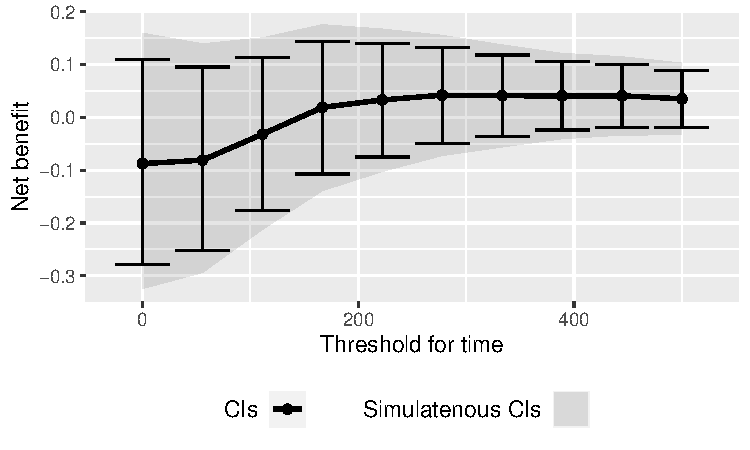
\includegraphics[width=0.5\textwidth]{./figures/gg-sensitivity1.pdf}
\end{center}

With multiple endpoints, the thresholds can be specified using a list:
\lstset{language=r,label= ,caption= ,captionpos=b,numbers=none}
\begin{lstlisting}
BTse.H <- sensitivity(BT.H, trace = FALSE,
		      threshold = list(time = seq(0,500,length = 10), karno = c(0,40,80)))
head(BTse.H)
\end{lstlisting}

\begin{verbatim}
       time karno    estimate         se   lower.ci   upper.ci null   p.value
1   0.00000     0 -0.08754474 0.10044847 -0.2786016 0.11017738    0 0.3858987
2  55.55556     0 -0.11177487 0.09915501 -0.2995661 0.08435417    0 0.2636263
3 111.11111     0 -0.08618872 0.09822940 -0.2732475 0.10715096    0 0.3826244
4 166.66667     0 -0.05180121 0.09818252 -0.2400240 0.14017526    0 0.5984319
5 222.22222     0 -0.03668720 0.09810141 -0.2253052 0.15458146    0 0.7086747
6 277.77778     0 -0.02906324 0.09773146 -0.2172647 0.16122161    0 0.7663054
\end{verbatim}


or a matrix:

\lstset{language=r,label= ,caption= ,captionpos=b,numbers=none}
\begin{lstlisting}
grid <- expand.grid(list("time_t20" = seq(0,500,length = 10), "karno" = c(0,40,80)))
cbind(head(grid)," " = "  ...   ",tail(grid))
BTse.H2 <-sensitivity(BT.H, threshold = grid, trace = FALSE)
range(BTse.H-BTse.H2)
\end{lstlisting}

\begin{verbatim}
   time_t20 karno          time_t20 karno
1   0.00000     0   ...    222.2222    80
2  55.55556     0   ...    277.7778    80
3 111.11111     0   ...    333.3333    80
4 166.66667     0   ...    388.8889    80
5 222.22222     0   ...    444.4444    80
6 277.77778     0   ...    500.0000    80
[1] 0 0
\end{verbatim}


The latter should be used when the same endpoint is used at different
priorities (each column correspond to the threshold that should be
used at a priority). As before we can display the results using the
autoplot function:
\lstset{language=r,label= ,caption= ,captionpos=b,numbers=none}
\begin{lstlisting}
autoplot(BTse.H, col = NA)
##  alternative display:
## autoplot(BTse.H, position  = position_dodge(width = 15))
\end{lstlisting}

\begin{center}
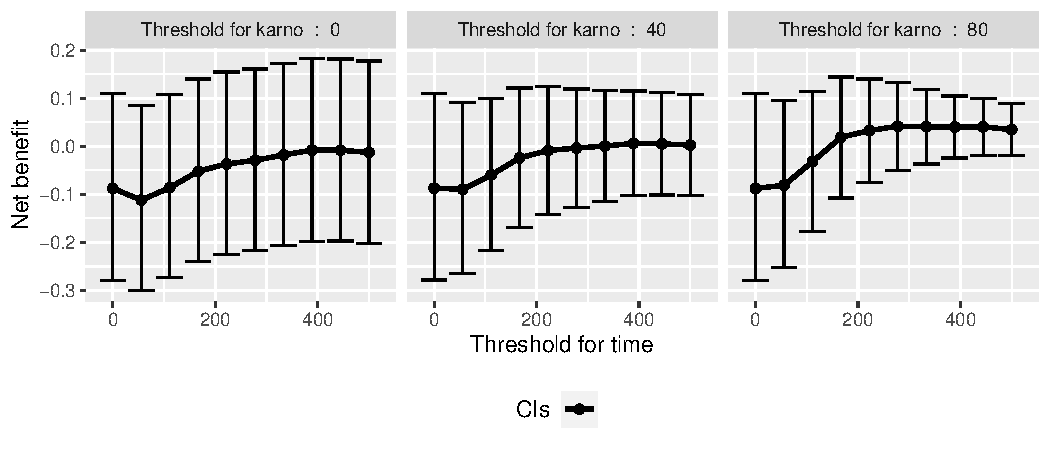
\includegraphics[width=\textwidth]{./figures/gg-sensitivity2.pdf}
\end{center}

Note that the autoplot function cannot be used when more than 2
thresholds are varied at the same time.

\section{Getting additional inside: looking at the pair level}
\label{sec:orgd90bcd8}

So far we have looked at the overall score and probabilities. But it
is also possible to extract the score relative to each pair, as well
as to "manually" compute this score. This can give further inside on
what the software is actually doing and what is the contribution of
each individual on the evaluation of the treatment.

\subsection{Extracting the contribution of each pair to the statistic}
\label{sec:orga6e260a}
The net benefit or the win ratio statistics can be expressed as a sum
of a score over all pairs of patients. The argument \texttt{keep.pairScore}
enables to export the score relative to each pair in the output of
BuyseTest:
\lstset{language=r,label= ,caption= ,captionpos=b,numbers=none}
\begin{lstlisting}
form <- trt ~ tte(time, threshold = 20, status = "status") + cont(karno)
BT.keep <- BuyseTest(form,
		     data = veteran, keep.pairScore = TRUE, 
		     trace = 0, method.inference = "none")
\end{lstlisting}

The method \texttt{getPairScore} can then be used to extract the contribution
of each pair. For instance the following code extracts the
contribution for the first endpoint:
\lstset{language=r,label= ,caption= ,captionpos=b,numbers=none}
\begin{lstlisting}
getPairScore(BT.keep, endpoint = 1)
\end{lstlisting}

\begin{verbatim}
      index.1 index.2 favorable unfavorable neutral uninf weight
   1:       1      70         1           0       0     0      1
   2:       2      70         1           0       0     0      1
   3:       3      70         1           0       0     0      1
   4:       4      70         1           0       0     0      1
   5:       5      70         1           0       0     0      1
  ---                                                           
4688:      65     137         0           1       0     0      1
4689:      66     137         0           1       0     0      1
4690:      67     137         0           1       0     0      1
4691:      68     137         0           1       0     0      1
4692:      69     137         0           1       0     0      1
\end{verbatim}

Each line corresponds to different comparison between a pair from the
control arm and the treatment arm. The column \texttt{strata} store to which
strata the pair belongs (first, second, \ldots{}). The columns favorable,
unfavorable, neutral, uninformative contains the result of the
comparison, e.g. the first pair was classified as favorable while the
last was classified as favorable with a weight of 1. The second and
third columns indicates the rows in the original dataset corresponding
to the pair:
\lstset{language=r,label= ,caption= ,captionpos=b,numbers=none}
\begin{lstlisting}
veteran[c(70,1),]
\end{lstlisting}

\begin{verbatim}
   trt celltype time status karno diagtime age prior
70   2 squamous  999      1    90       12  54    10
1    1 squamous   72      1    60        7  69     0
\end{verbatim}



For the first pair, the event was observed for both observations and
since 999 > 72 + 20 the pair is rated favorable. Substracting the
average probability of the pair being favorable minus the average
probability of the pair being unfavorable:
\lstset{language=r,label= ,caption= ,captionpos=b,numbers=none}
\begin{lstlisting}
getPairScore(BT.keep, endpoint = 1)[, mean(favorable) - mean(unfavorable)]
\end{lstlisting}

\begin{verbatim}
[1] -0.08765836
\end{verbatim}


gives the net benefit in favor of the treatment for the first
endpoint:
\lstset{language=r,label= ,caption= ,captionpos=b,numbers=none}
\begin{lstlisting}
BT.keep
\end{lstlisting}

\begin{verbatim}
endpoint threshold   delta   Delta
    time        20 -0.0877 -0.0877
   karno           -0.0133 -0.1009
\end{verbatim}


More examples and explanation can be found in the documentation of
the method \texttt{getPairScore}.

\subsection{Extracting the survival probabilities}
\label{sec:orgc966105}
When using \texttt{scoring.rule} equals \texttt{"Peron"}, survival probabilities at
event time, and event times +/- threshold in the control and treatment
arms are used to score the pair. Setting \texttt{keep.survival} to \texttt{TRUE} and
\texttt{precompute} to \texttt{FALSE} in BuyseTest.options enables to export the
survival probabilities in the output of BuyseTest:
\lstset{language=r,label= ,caption= ,captionpos=b,numbers=none}
\begin{lstlisting}
BuyseTest.options(keep.survival = TRUE, precompute = FALSE)
BT.keep2 <- BuyseTest(trt ~ tte(time, threshold = 20, status = "status") + cont(karno),
		      data = veteran, keep.pairScore = TRUE, scoring.rule = "Peron",
		      trace = 0, method.inference = "none")
\end{lstlisting}

The method \texttt{getSurvival} can then be used to extract these survival
probabilities. For instance the following code extracts the survival
for the first endpoint:
\lstset{language=r,label= ,caption= ,captionpos=b,numbers=none}
\begin{lstlisting}
outSurv <- getSurvival(BT.keep2, endpoint = 1, strata = 1)
str(outSurv)
\end{lstlisting}

\begin{verbatim}
List of 5
 $ survTimeC: num [1:69, 1:13] 72 411 228 126 118 10 82 110 314 100 ...
  ..- attr(*, "dimnames")=List of 2
  .. ..$ : NULL
  .. ..$ : chr [1:13] "time" "survivalC-threshold" "survivalC_0" "survivalC+threshold" ...
 $ survTimeT: num [1:68, 1:13] 999 112 87 231 242 991 111 1 587 389 ...
  ..- attr(*, "dimnames")=List of 2
  .. ..$ : NULL
  .. ..$ : chr [1:13] "time" "survivalC-threshold" "survivalC_0" "survivalC+threshold" ...
 $ survJumpC: num [1:57, 1:6] 3 4 7 8 10 11 12 13 16 18 ...
  ..- attr(*, "dimnames")=List of 2
  .. ..$ : NULL
  .. ..$ : chr [1:6] "time" "survival" "dSurvival" "index.survival" ...
 $ survJumpT: num [1:51, 1:6] 1 2 7 8 13 15 18 19 20 21 ...
  ..- attr(*, "dimnames")=List of 2
  .. ..$ : NULL
  .. ..$ : chr [1:6] "time" "survival" "dSurvival" "index.survival" ...
 $ lastSurv : num [1:2] 0 0
\end{verbatim}

\subsubsection{Computation of the score with only one censored event}
\label{sec:orge5ef305}

Let's look at pair 91:
\lstset{language=r,label= ,caption= ,captionpos=b,numbers=none}
\begin{lstlisting}
getPairScore(BT.keep2, endpoint = 1, rm.withinStrata = FALSE)[91]
\end{lstlisting}

\begin{verbatim}
   index.1 index.2 indexWithinStrata.1 indexWithinStrata.2 favorable unfavorable   neutral
1:      22      71                  22                   2         0   0.6950827 0.3049173
   uninf weight
1:     0      1
\end{verbatim}


In the dataset this corresponds to:
\lstset{language=r,label= ,caption= ,captionpos=b,numbers=none}
\begin{lstlisting}
veteran[c(22,71),]
\end{lstlisting}

\begin{verbatim}
   trt  celltype time status karno diagtime age prior
22   1 smallcell   97      0    60        5  67     0
71   2  squamous  112      1    80        6  60     0
\end{verbatim}


The observation from the control group is censored at 97 while the
observation from the treatment group has an event at 112. Since the
threshold is 20, and (112-20)<97, we know that the pair is not in
favor of the treatment. The formula for probability in favor of the
control is \(\frac{S_c(97)}{S_c(112+20)}\). The survival at the event
time in the censoring group is stored in survTimeC. Since observation
22 is the 22th observation in the control group:
\lstset{language=r,label= ,caption= ,captionpos=b,numbers=none}
\begin{lstlisting}
iSurv <- outSurv$survTimeC[22,] 
iSurv
\end{lstlisting}

\begin{verbatim}
                     time       survivalC-threshold               survivalC_0 
               97.0000000                 0.5615232                 0.5171924 
      survivalC+threshold       survivalT-threshold               survivalT_0 
                0.4235463                 0.4558824                 0.3643277 
      survivalT+threshold index.survivalC-threshold         index.survivalC_0 
                0.2827500                25.0000000                28.0000000 
index.survivalC+threshold index.survivalT-threshold         index.survivalT_0 
               33.0000000                27.0000000                32.0000000 
index.survivalT+threshold 
               35.0000000
\end{verbatim}

Since we are interested in the survival in the control arm exactly at the event time:
\lstset{language=r,label= ,caption= ,captionpos=b,numbers=none}
\begin{lstlisting}
Sc97 <- iSurv["survivalC_0"] 
Sc97
\end{lstlisting}

\begin{verbatim}
survivalC_0 
  0.5171924
\end{verbatim}


The survival at the event time in the treatment group is stored in
survTimeC. Since observation 71 is the 2nd observation in the treatment
group:
\lstset{language=r,label= ,caption= ,captionpos=b,numbers=none}
\begin{lstlisting}
iSurv <- outSurv$survTimeT[2,] ## survival at time 112+20
iSurv
\end{lstlisting}

\begin{verbatim}
                     time       survivalC-threshold               survivalC_0 
              112.0000000                 0.5319693                 0.4549201 
      survivalC+threshold       survivalT-threshold               survivalT_0 
                0.3594915                 0.3801681                 0.2827500 
      survivalT+threshold index.survivalC-threshold         index.survivalC_0 
                0.2827500                27.0000000                32.0000000 
index.survivalC+threshold index.survivalT-threshold         index.survivalT_0 
               37.0000000                31.0000000                35.0000000 
index.survivalT+threshold 
               35.0000000
\end{verbatim}

Since we are interested in the survival in the control arm at the event time plus threshold:
\lstset{language=r,label= ,caption= ,captionpos=b,numbers=none}
\begin{lstlisting}
Sc132 <- iSurv["survivalC+threshold"] 
Sc132
\end{lstlisting}

\begin{verbatim}
survivalC+threshold 
          0.3594915
\end{verbatim}


The probability in favor of the control is then:
\lstset{language=r,label= ,caption= ,captionpos=b,numbers=none}
\begin{lstlisting}
Sc132/Sc97
\end{lstlisting}

\begin{verbatim}
survivalC+threshold 
          0.6950827
\end{verbatim}

\subsubsection{Computation of the score with two censored events}
\label{sec:orga16256b}

When both observations are censored, the formula for computing the
probability in favor of treatment or control involves an
integral. This integral can be computed using the function
\texttt{calcIntegralSurv\textbackslash{}\_cpp} that takes as argument a matrix containing the
survival and the jumps in survival, e.g.:
\lstset{language=r,label= ,caption= ,captionpos=b,numbers=none}
\begin{lstlisting}
head(outSurv$survJumpT)
\end{lstlisting}

\begin{verbatim}
     time  survival   dSurvival index.survival index.dsurvival1 index.dsurvival2
[1,]    1 0.7681159 -0.02941176             12                0                1
[2,]    2 0.7536232 -0.01470588             13                1                2
[3,]    7 0.7388463 -0.02941176             14                2                3
[4,]    8 0.7388463 -0.02941176             14                3                4
[5,]   13 0.7092924 -0.01470588             16                4                5
[6,]   15 0.6945155 -0.02941176             17                5                6
\end{verbatim}


and the starting time of the integration time. For instance, let's
look at pair 148:
\lstset{language=r,label= ,caption= ,captionpos=b,numbers=none}
\begin{lstlisting}
getPairScore(BT.keep2, endpoint = 1, rm.withinStrata = FALSE)[148]
\end{lstlisting}

\begin{verbatim}
   index.1 index.2 indexWithinStrata.1 indexWithinStrata.2 favorable unfavorable   neutral
1:      10      72                  10                   3 0.5058685   0.3770426 0.1170889
   uninf weight
1:     0      1
\end{verbatim}


which corresponds to the observations:
\lstset{language=r,label= ,caption= ,captionpos=b,numbers=none}
\begin{lstlisting}
veteran[c(10,72),]
\end{lstlisting}

\begin{verbatim}
   trt celltype time status karno diagtime age prior
10   1 squamous  100      0    70        6  70     0
72   2 squamous   87      0    80        3  48     0
\end{verbatim}


The probability in favor of the treatment (\(p_F\)) and control (\(p_{UF}\)) can be computed
as:
\begin{align*}
p_F &= -\frac{1}{S_T(x)S_C(y)}\int_{t>y} S_T(t+\tau) dS_C(t) \\
p_{UF} &= -\frac{1}{S_T(x)S_C(y)}\int_{t>x} S_C(t+\tau) dS_T(t)
\end{align*}
where \(x=87\) and \(y=100\). To ease the call of \texttt{calcIntegralScore\_cpp} we create a warper:
\lstset{language=r,label= ,caption= ,captionpos=b,numbers=none}
\begin{lstlisting}
calcInt <- function(...){ ## no need for the functionnal derivative of the score 
    BuyseTest:::.calcIntegralSurv_cpp(..., 
				      returnDeriv = FALSE, 
				      derivSurv = matrix(0), 
				      derivSurvD = matrix(0))
}
\end{lstlisting}

and then call it to compute the probabilities:
\lstset{language=r,label= ,caption= ,captionpos=b,numbers=none}
\begin{lstlisting}
denom <- as.double(outSurv$survTimeT[3,"survivalT_0"] * outSurv$survTimeC[10,"survivalC_0"])
M <- cbind("favorable" = -calcInt(outSurv$survJumpC, start = 100, 
				  lastSurv = outSurv$lastSurv[2],
				  lastdSurv = outSurv$lastSurv[1])/denom,
	   "unfavorable" = -calcInt(outSurv$survJumpT, start = 87, 
				    lastSurv = outSurv$lastSurv[1],
				    lastdSurv = outSurv$lastSurv[2])/denom)
rownames(M) <- c("lowerBound","upperBound")
M
\end{lstlisting}

\begin{verbatim}
           favorable unfavorable
lowerBound 0.5058685   0.3770426
upperBound 0.5058685   0.3770426
\end{verbatim}


Note: the lower bound is identical to the upper bound as we could
estimate the full survival curve:
\lstset{language=r,label= ,caption= ,captionpos=b,numbers=none}
\begin{lstlisting}
outSurv$lastSurv
\end{lstlisting}

\begin{verbatim}
[1] 0 0
\end{verbatim}


\clearpage

\section{Dealing with missing values or/and right censoring}
\label{sec:org2d9dcf3}

In presence of censoring or missing values, it is often not be
 possible to classify all pairs without a model for the censoring
 mechanism. The unclassified pairs, called uninformative, have a score
 of 0 which will typically bias the estimate of the net net benefit
 towards 0 \footnote{While the power is typically reduced, the type 1 error
 will still be controled if censoring is at random}. Consider the
 following dataset:
\lstset{language=r,label= ,caption= ,captionpos=b,numbers=none}
\begin{lstlisting}
set.seed(10)
dt <- simBuyseTest(1e2, latent = TRUE, argsCont = NULL,
		   argsTTE = list(scale.T = 1/2, scale.C = 1,
				  scale.Censoring.C = 1, scale.Censoring.T = 1))
dt[, eventtimeCensoring := NULL]
dt[, status1 := 1]
head(dt)
\end{lstlisting}

\begin{verbatim}
   treatment eventtimeUncensored eventtime status toxicity eta_toxicity status1
1:         C           0.2135567 0.2135567      1      yes  -0.07945702       1
2:         C           0.3422379 0.3422379      1       no   1.18175155       1
3:         C           1.3933222 1.3933222      1       no   2.18614406       1
4:         C           0.6737702 0.1961599      0       no   0.40617493       1
5:         C           0.5642992 0.5642992      1      yes  -0.73835910       1
6:         C           1.1039218 0.1764950      0      yes  -1.95648670       1
\end{verbatim}


where we have the uncensored event times (\texttt{eventtimeUncensored}) as well as the censored event
times (\texttt{eventtime}). The percentage of censored observations is:
\lstset{language=r,label= ,caption= ,captionpos=b,numbers=none}
\begin{lstlisting}
100*dt[,mean(status==0)]
\end{lstlisting}

\begin{verbatim}
[1] 44
\end{verbatim}


We would like to be able to recover the net benefit estimated with the uncensored event times:
\lstset{language=r,label= ,caption= ,captionpos=b,numbers=none}
\begin{lstlisting}
BuyseTest(treatment ~ tte(eventtimeUncensored, status1, threshold = 0.5),
	  data = dt,
	  scoring.rule = "Gehan", method.inference = "none", trace = 0)
\end{lstlisting}

\begin{verbatim}
           endpoint threshold  Delta
eventtimeUncensored       0.5 -0.271
\end{verbatim}


using the censored survival times.

\clearpage

The \texttt{BuyseTest} function handles missing values via two arguments:
\begin{itemize}
\item \texttt{scoring.rule} indicates how pairs involving missing data are compared. 
\begin{itemize}
\item \textbf{the Gehan's scoring rule} compares the observed values. If it is
not possible to decide whether one observation has a better
endpoint than the other (e.g. because both are right-censoring)
then the paired is scored uninformative.
\item \textbf{the Peron's scoring rule} compares the probabilty of one
observation having a better endpoint than the other given the
observed values. This require a model for the censoring
distribution. If the full survival curve can be identified then
all pairs can be fully classified otherwise some of the pair
will be partially uninformative.
\end{itemize}
\item \texttt{correction.uninf} indicates what to do with the uninformative
scores. Setting this argument to \texttt{TRUE} will re-distribute this
score to favorable/unfavorable/neutral scores.
\end{itemize}

When the survival curve can be fully identified, the default (and
recommanded) approach is to use the Peron's scoring rule where the
censoring model rely on Kaplan Meier curve is fitted in each treatment
group. When the last observation are censored, then part of the
survival curve is unknown and there is no perfect solution. One can:
\begin{itemize}
\item only use the Peron's scoring rule, which will lead to a non-0
uninformative score and therefore a "conservative" estimate of the net benefit.
\item use the Peron's scoring rule in conjonction with the correction
which will led to an unbiased estimator if certain assumption are met.
\item only use the Peron's scoring rule with a parametric model which, if
appropriate, will lead to an unbiased (and rather efficient)
estimator.
\end{itemize}

\subsection{Gehan's scoring rule}
\label{sec:org429dfc9}
In the example, Gehan's scoring rule:
\lstset{language=r,label= ,caption= ,captionpos=b,numbers=none}
\begin{lstlisting}
e.G <- BuyseTest(treatment ~ tte(eventtime, status, threshold = 0.5),
	  data = dt, scoring.rule = "Gehan", trace = 0)
summary(e.G, print=FALSE)$table.print
\end{lstlisting}

\begin{verbatim}
   endpoint threshold total(%) favorable(%) unfavorable(%) neutral(%) uninf(%)   Delta
1 eventtime       0.5      100         4.67          14.39      20.44     60.5 -0.0972
  CI [2.5% ; 97.5%]   p.value significance
1 [-0.1594;-0.0342] 0.0025149           **
\end{verbatim}


leads to many uninformative pairs (about 60\%) and an estimate much
closer to 0 than the truth.

\subsection{Peron's scoring rule}
\label{sec:org4c33b49}
In the example, Peron's scoring rule:
\lstset{language=r,label= ,caption= ,captionpos=b,numbers=none}
\begin{lstlisting}
e.P <- BuyseTest(treatment ~ tte(eventtime, status, threshold = 0.5),
	  data = dt, scoring.rule = "Peron", trace = 0)
summary(e.P, print=FALSE)$table.print
\end{lstlisting}

\begin{verbatim}
   endpoint threshold total(%) favorable(%) unfavorable(%) neutral(%) uninf(%)   Delta
1 eventtime       0.5      100        11.17          43.34      44.12     1.37 -0.3216
  CI [2.5% ; 97.5%]    p.value significance
1   [-0.4584;-0.17] 5.3851e-05          ***
\end{verbatim}

leads to no uninformative pairs. Indeed the last observation in each group is an (uncensored) event:
\lstset{language=r,label= ,caption= ,captionpos=b,numbers=none}
\begin{lstlisting}
dt[,.SD[which.max(eventtime)],by="treatment"]
\end{lstlisting}

\begin{verbatim}
   treatment eventtimeUncensored eventtime status toxicity eta_toxicity status1
1:         C            2.668629  2.668629      1      yes   -1.9256436       1
2:         T            1.674053  1.588657      0      yes   -0.8647272       1
\end{verbatim}

so the full survival curve could be identified. As a result the estimate is very close to the
truth. 

\bigskip

\uline{Note 1:} the censoring model can be specified by first fitting a
Kaplan Meier model for the survival time:
\lstset{language=r,label= ,caption= ,captionpos=b,numbers=none}
\begin{lstlisting}
library(prodlim)
e.prodlim <- prodlim(Hist(eventtime, status) ~ treatment, data = dt)
\end{lstlisting}

Then passing the model to the \texttt{BuyseTest} via the \texttt{model.tte} argument:
\lstset{language=r,label= ,caption= ,captionpos=b,numbers=none}
\begin{lstlisting}
e.P1 <- BuyseTest(treatment ~ tte(eventtime, status, threshold = 0.5),
		  model.tte = e.prodlim,
		  data = dt, scoring.rule = "Peron", trace = 0)
summary(e.P1, print=FALSE)$table.print
\end{lstlisting}

\begin{verbatim}
   endpoint threshold total(%) favorable(%) unfavorable(%) neutral(%) uninf(%)   Delta
1 eventtime       0.5      100        11.17          43.34      44.12     1.37 -0.3216
  CI [2.5% ; 97.5%]    p.value significance
1 [-0.4187;-0.2173] 6.5701e-09          ***
\end{verbatim}


Note that the CI/p-value have changed since, unless stated otherwise,
\texttt{BuyseTest} assumes no uncertainty about the survival model when using
\texttt{model.tte}. One can force it to account for the uncertainty adding an attribute:
\lstset{language=r,label= ,caption= ,captionpos=b,numbers=none}
\begin{lstlisting}
attr(e.prodlim, "iidNuisance") <- TRUE
e.P2 <- BuyseTest(treatment ~ tte(eventtime, status, threshold = 0.5),
		  model.tte = e.prodlim,
		  data = dt, scoring.rule = "Peron", trace = 0)
summary(e.P2, print=FALSE)$table.print
\end{lstlisting}

\begin{verbatim}
   endpoint threshold total(%) favorable(%) unfavorable(%) neutral(%) uninf(%)   Delta
1 eventtime       0.5      100        11.17          43.34      44.12     1.37 -0.3216
  CI [2.5% ; 97.5%]    p.value significance
1   [-0.4584;-0.17] 5.3851e-05          ***
\end{verbatim}


\bigskip

\uline{Note 2:} it is possible to use a parametric model via the \texttt{survreg} function:
\lstset{language=r,label= ,caption= ,captionpos=b,numbers=none}
\begin{lstlisting}
library(survival)
e.survreg <- survreg(Surv(eventtime, status) ~ treatment, data = dt, 
		     dist = "weibull")
attr(e.survreg, "iidNuisance") <- TRUE
\end{lstlisting}

Then passing the model to the \texttt{BuyseTest} via the \texttt{model.tte} argument:
\lstset{language=r,label= ,caption= ,captionpos=b,numbers=none}
\begin{lstlisting}
e.P3 <- BuyseTest(treatment ~ tte(eventtime, status, threshold = 0.5),
		  model.tte = e.survreg,
		  data = dt, scoring.rule = "Peron", trace = 0)
summary(e.P3, print=FALSE)$table.print
\end{lstlisting}
\begin{verbatim}
   endpoint threshold total(%) favorable(%) unfavorable(%) neutral(%) uninf(%)   Delta
1 eventtime       0.5      100        11.88          34.19      53.92     0.01 -0.2231
  CI [2.5% ; 97.5%]    p.value significance
1 [-0.3455;-0.0932] 0.00085702          ***
\end{verbatim}


Internally the survival curve is discretized using 1000 points
starting from survival = 1 to survival = 0.001 (this is why there is a
non-0 but small percentage of uninformative pairs). This is performed
internally by applying the \texttt{BuyseTTEM} method. Another discretisation
can be obtained by calling \texttt{BuyseTTEM} with another value for the \texttt{n.grid} argument:
\lstset{language=r,label= ,caption= ,captionpos=b,numbers=none}
\begin{lstlisting}
e.TTEM <- BuyseTTEM(e.survreg, treatment = "treatment", iid = TRUE, n.grid = 2500)
attr(e.TTEM, "iidNuisance") <- TRUE
str(e.TTEM$peron$jumpSurvHaz[[1]][[1]])
\end{lstlisting}

\begin{verbatim}
'data.frame':	2500 obs. of  3 variables:
 $ index.jump: logi  NA NA NA NA NA NA ...
 $ time.jump : num  0 0.000307 0.000632 0.000964 0.001301 ...
 $ survival  : num  1 1 0.999 0.999 0.998 ...
\end{verbatim}


and then passing to \texttt{BuyseTest}:
\lstset{language=r,label= ,caption= ,captionpos=b,numbers=none}
\begin{lstlisting}
e.P4 <- BuyseTest(treatment ~ tte(eventtime, status, threshold = 0.5),
		  model.tte = e.TTEM,
		  data = dt, scoring.rule = "Peron", trace = 0)
summary(e.P4, print=FALSE)$table.print
\end{lstlisting}

\begin{verbatim}
   endpoint threshold total(%) favorable(%) unfavorable(%) neutral(%) uninf(%)   Delta
1 eventtime       0.5      100        11.87          34.18      53.94     0.01 -0.2231
  CI [2.5% ; 97.5%]    p.value significance
1 [-0.3455;-0.0932] 0.00085776          ***
\end{verbatim}


It is therefore possible to extend the approach to other model by
defining an appropriate \texttt{BuyseTTEM} method. Looking at the code use
for defining \texttt{BuyseTTEM.survreg} can be helpful.

\subsection{Correction via inverse probability-of-censoring weights (IPCW)}
\label{sec:org0f29cc7}

With IPCW, the weights of the non-informative pairs is redistributed
to the informative pairs. This is only a good strategy when there are
no neutral pairs or there are no lower priority endpoints. This gives
an estimate much closer to the true net benefit:
\lstset{language=r,label= ,caption= ,captionpos=b,numbers=none}
\begin{lstlisting}
BT <- BuyseTest(treatment ~ tte(eventtime, status, threshold = 0.5),
		data = dt, keep.pairScore = TRUE, trace = 0,
		scoring.rule = "Gehan", method.inference = "none", correction.uninf = 2)
summary(BT)
\end{lstlisting}

\begin{verbatim}
      Generalized pairwise comparisons with 1 endpoint

- statistic       : net benefit (delta: endpoint specific, Delta: global) 
- null hypothesis : Delta == 0 
- treatment groups: T (treatment) vs. C (control) 
- censored pairs  : deterministic score or uninformative
- uninformative pairs: no contribution, their weight is passed to the informative pairs using IPCW
- results
 endpoint threshold total(%) favorable(%) unfavorable(%) neutral(%) uninf(%)   Delta
eventtime       0.5      100        11.82          36.43      51.75        0 -0.2461
\end{verbatim}


We can also see that no pair is finally classified as non
informative. To get some inside about the correction we can look at
the scores of the pairs:
\lstset{language=r,label= ,caption= ,captionpos=b,numbers=none}
\begin{lstlisting}
iScore <- getPairScore(BT, endpoint = 1)
\end{lstlisting}

To get a synthetic view, we only look at the unique
favorable/unfavorable/neutral/uniformative results:
\lstset{language=r,label= ,caption= ,captionpos=b,numbers=none}
\begin{lstlisting}
iScore[,.SD[1], 
       .SDcols = c("favorableC","unfavorableC","neutralC","uninfC"),
       by = c("favorable","unfavorable","neutral","uninf")]
\end{lstlisting}

\begin{verbatim}
   favorable unfavorable neutral uninf favorableC unfavorableC neutralC uninfC
1:         0           0       1     0   0.000000     0.000000 2.531646      0
2:         0           1       0     0   0.000000     2.531646 0.000000      0
3:         0           0       0     1   0.000000     0.000000 0.000000      0
4:         1           0       0     0   2.531646     0.000000 0.000000      0
\end{verbatim}


We can see that the favorable/unfavorable/neutral pairs have seen
their contribution multiplied by:
\lstset{language=r,label= ,caption= ,captionpos=b,numbers=none}
\begin{lstlisting}
iScore[,1/mean(favorable + unfavorable + neutral)]
\end{lstlisting}

\begin{verbatim}
[1] 2.531646
\end{verbatim}


i.e. the inverse probability of being informative. 

\subsection{Correction at the pair level}
\label{sec:orga9f06bb}

Another possible correction is to distribute the non-informative
weight of a pair to the average favorable/unfavorable/neutral
probability observed on the sample:
\lstset{language=r,label= ,caption= ,captionpos=b,numbers=none}
\begin{lstlisting}
BT <- BuyseTest(treatment ~ tte(eventtime, status, threshold = 0.5),
		data = dt, keep.pairScore = TRUE, trace = 0,
		scoring.rule = "Gehan", method.inference = "none", correction.uninf = TRUE)
summary(BT)
\end{lstlisting}

\begin{verbatim}
      Generalized pairwise comparisons with 1 endpoint

- statistic       : net benefit (delta: endpoint specific, Delta: global) 
- null hypothesis : Delta == 0 
- treatment groups: T (treatment) vs. C (control) 
- censored pairs  : deterministic score or uninformative
- uninformative pairs: score equals the averaged score of all informative pairs
- results
 endpoint threshold total(%) favorable(%) unfavorable(%) neutral(%) uninf(%)   Delta
eventtime       0.5      100        11.82          36.43      51.75        0 -0.2461
\end{verbatim}


Looking at the scores of the pairs:
\lstset{language=r,label= ,caption= ,captionpos=b,numbers=none}
\begin{lstlisting}
iScore <- getPairScore(BT, endpoint = 1)
iScore[,.SD[1], 
       .SDcols = c("favorableC","unfavorableC","neutralC","uninfC"),
       by = c("favorable","unfavorable","neutral","uninf")]
\end{lstlisting}

\begin{verbatim}
   favorable unfavorable neutral uninf favorableC unfavorableC  neutralC uninfC
1:         0           0       1     0  0.0000000    0.0000000 1.0000000      0
2:         0           1       0     0  0.0000000    1.0000000 0.0000000      0
3:         0           0       0     1  0.1182278    0.3643038 0.5174684      0
4:         1           0       0     0  1.0000000    0.0000000 0.0000000      0
\end{verbatim}


we can see that the corrected probability have not changed for the
informative pairs, but for the non-informative they have been set to:
\lstset{language=r,label= ,caption= ,captionpos=b,numbers=none}
\begin{lstlisting}
iScore[, .(favorable = weighted.mean(favorable, w = 1-uninf), 
	   unfavorable = weighted.mean(unfavorable, w = 1-uninf), 
	   neutral = weighted.mean(neutral, w = 1-uninf))]
\end{lstlisting}

\begin{verbatim}
   favorable unfavorable   neutral
1: 0.1182278   0.3643038 0.5174684
\end{verbatim}

\subsection{Note on the use of the corrections}
\label{sec:org885d4bf}

As mentioned in \cite{peron2021correcting}, the corrections (at the pair
level or IPCW) are assumes that uninformative pairs would on average
behave like informative pairs. This is typically the case under the
proportional hazard assumption. However that may not be the case with
other distributions, e.g.:
\lstset{language=r,label= ,caption= ,captionpos=b,numbers=none}
\begin{lstlisting}
set.seed(10);n <- 250; 
df <- rbind(data.frame(group = "T1", time = rweibull(n, shape = 1, scale = 2), status = 1),
	    data.frame(group = "T2", time = rweibull(n, shape = 2, scale = 1.8), status = 1))
df$censoring <- runif(NROW(df),0,2)
df$timeC <- pmin(df$time,df$censoring)
df$statusC <- as.numeric(df$time<=df$censoring)
plot(prodlim(Hist(time,status)~group, data = df)); title("complete data");
plot(prodlim(Hist(timeC,statusC)~group, data = df)); title("right-censored data");
\end{lstlisting}
\begin{center}
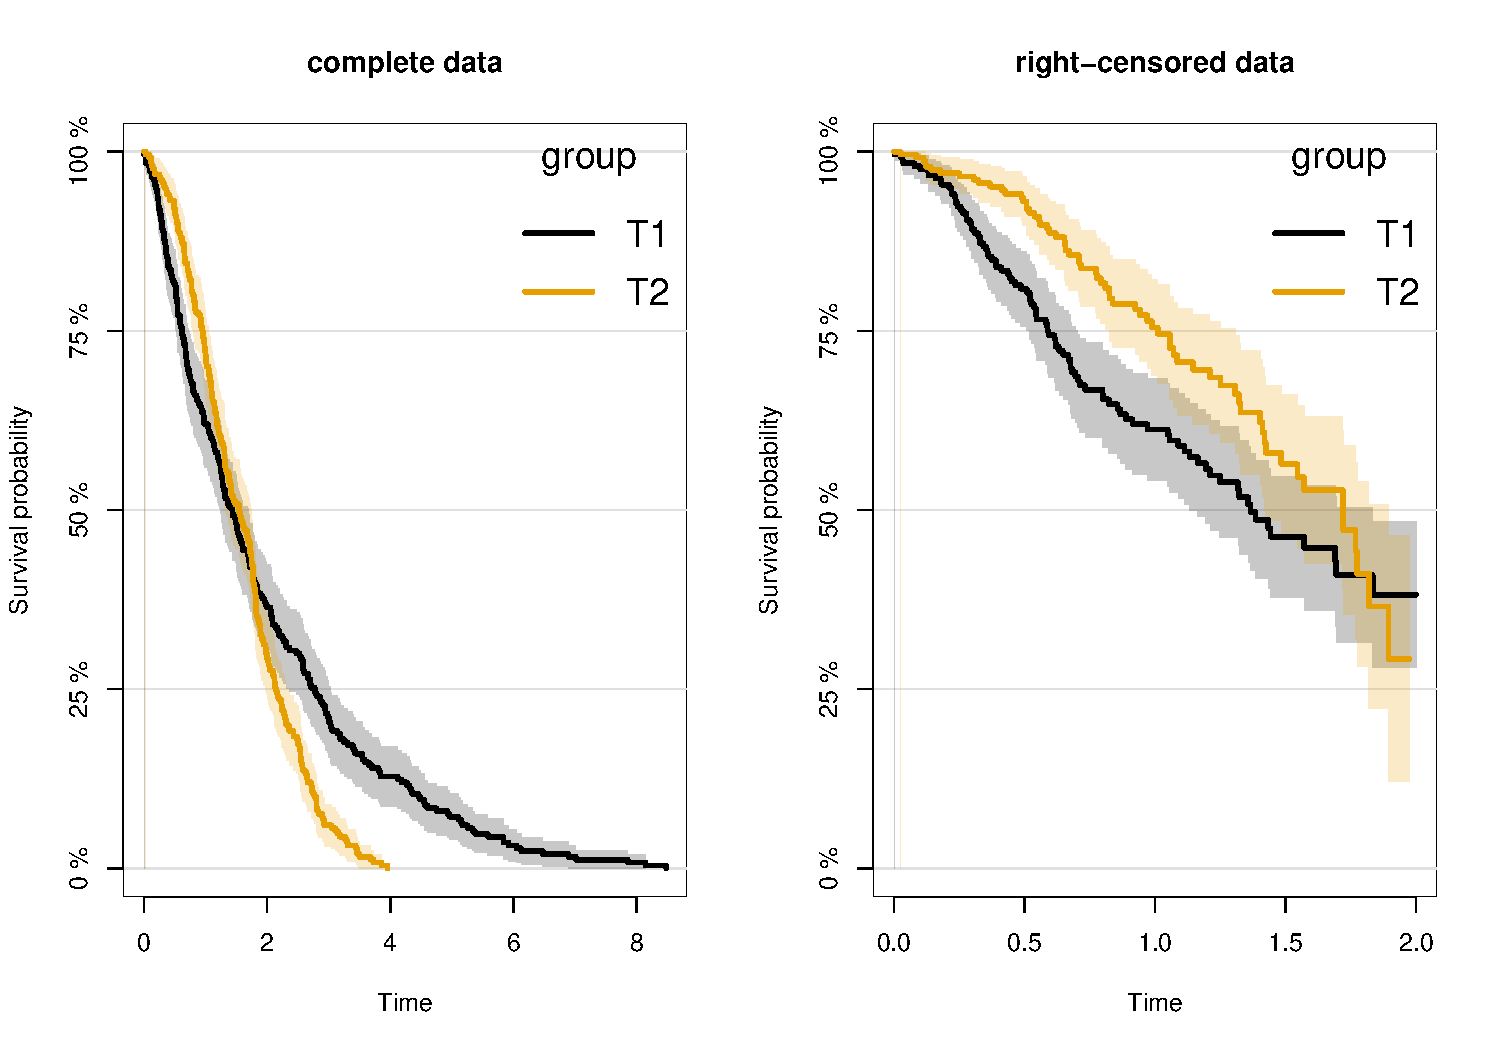
\includegraphics[width=0.8\textwidth]{./figures/plot-crossingSurv.pdf}
\end{center}

Here the net benefit that we would have estimated with complete data:
\lstset{language=r,label= ,caption= ,captionpos=b,numbers=none}
\begin{lstlisting}
BuyseTest.options(method.inference = "none")
e.ref <- BuyseTest(group ~ tte(time,status), data = df, trace = FALSE)
s.ref <- summary(e.ref, print = FALSE)$table[1,c("favorable","unfavorable","neutral","uninf","Delta")]
s.ref
\end{lstlisting}

\begin{verbatim}
  favorable unfavorable neutral uninf    Delta
1   50.2048     49.7952       0     0 0.004096
\end{verbatim}


can be taken as a reference. Violation of the assumption will in this
example have a substantial impact and lead to a worse estimate with
the correction:
\lstset{language=r,label= ,caption= ,captionpos=b,numbers=none}
\begin{lstlisting}
e.correction <- BuyseTest(group ~ tte(timeC,statusC)+cont(time), data = df, trace = FALSE, correction.uninf = TRUE)
s.correction <- summary(e.correction, print = FALSE)$table[1,c("favorable","unfavorable","neutral","uninf","Delta")]
\end{lstlisting}

\begin{verbatim}
Warning message:
In .BuyseTest(envir = envirBT, iid = outArgs$iid, method.inference = "none",  :
  Some of the survival curves for endpoint(s) "timeC" are unknown beyond a survival of 0.25.
The correction of uninformative pairs assume that uninformative pairs would on average behave like informative pairs. 
This can be a strong assumption and have substantial impact when the tail of the survival curve is unknown.
\end{verbatim}


than without:
\lstset{language=r,label= ,caption= ,captionpos=b,numbers=none}
\begin{lstlisting}
e.Peron <- BuyseTest(group ~ tte(timeC,statusC), data = df, trace = FALSE)
s.Peron <- summary(e.Peron,print = FALSE)$table[1,c("favorable","unfavorable","neutral","uninf","Delta")]
rbind("reference" = s.ref,
      "no correction" = s.Peron,
      "correction" = s.correction)
\end{lstlisting}
\begin{verbatim}
              favorable unfavorable neutral    uninf      Delta
reference      50.20480    49.79520       0  0.00000 0.00409600
no correction  49.09253    39.74775       0 11.15972 0.09344778
correction     55.25931    44.74069       0  0.00000 0.10518628
\end{verbatim}


\clearpage

\section{Simulating data using \texttt{simBuyseTest}}
\label{sec:org7d32d87}
You can simulate data with the \texttt{simBuyseTest} function. For instance
the following code simulates data for 5 individuals in the treatment
arm and 5 individuals in the control arm:
\lstset{language=r,label= ,caption= ,captionpos=b,numbers=none}
\begin{lstlisting}
set.seed(10)
simBuyseTest(n.T = 5, n.C = 5)
\end{lstlisting}

\begin{verbatim}
    treatment  eventtime status toxicity       score
 1:         C 0.60539304      0      yes -1.85374045
 2:         C 0.31328027      1      yes -0.07794607
 3:         C 0.03946623      0      yes  0.96856634
 4:         C 0.32147489      1      yes  0.18492596
 5:         C 1.57044952      0      yes -1.37994358
 6:         T 0.29069131      0       no  1.10177950
 7:         T 0.19522131      0      yes  0.75578151
 8:         T 0.04640668      0      yes -0.23823356
 9:         T 0.05277335      1      yes  0.98744470
10:         T 0.43062009      1      yes  0.74139013
\end{verbatim}

By default a categorical, continuous and time to event outcome are
generated independently. You can modify their distribution via the
arguments \texttt{argsBin}, \texttt{argsCont}, \texttt{argsTTE}. For instance the following
code simulates two continuous variables with mean 5 in the treatment
arm and 10 in the control arm all with variance 1:
\lstset{language=r,label= ,caption= ,captionpos=b,numbers=none}
\begin{lstlisting}
set.seed(10)
argsCont <- list(mu.T = c(5,5), mu.C = c(10,10), 
		 sigma.T = c(1,1), sigma.C = c(1,1),
		 name = c("tumorSize","score"))
dt <- simBuyseTest(n.T = 5, n.C = 5,
		   argsCont = argsCont)
dt
\end{lstlisting}

\begin{verbatim}
    treatment eventtime status toxicity tumorSize     score
 1:         C 0.1805891      0      yes 11.086551  8.564486
 2:         C 0.1702538      1      yes  9.237455 10.362087
 3:         C 0.2621793      1       no  9.171337  8.240913
 4:         C 0.2959301      0       no 10.834474  9.675456
 5:         C 0.4816549      1      yes  9.032348  9.348437
 6:         T 0.6446131      1       no  5.089347  6.101780
 7:         T 0.7372264      1      yes  4.045056  5.755782
 8:         T 0.7213402      0      yes  4.804850  4.761766
 9:         T 0.1580651      1      yes  5.925521  5.987445
10:         T 0.2212117      0      yes  5.482979  5.741390
\end{verbatim}

This functionality is based on the \texttt{sim} function of the \textbf{lava}
package (\url{https://github.com/kkholst/lava})

\clearpage

\section{Power calculation using \texttt{powerBuyseTest}}
\label{sec:org09ef445}

The function \texttt{powerBuyseTest} can be used to perform power
calculation, i.e., estimate the probability of rejecting a null
hypothesis under a specific generative mechanism. The user therefore
need to specify:
\begin{itemize}
\item the generative mechanism via a function \hfill - argument \texttt{sim}
\item the null hypothesis \hfill - argument \texttt{null}
\item the sample size(s) for the which the power should be computed  \hfill - argument \texttt{sample.size}
\end{itemize}

\bigskip

Consider the following generative mechanism where the outcome follows
a Student's t-distribution in the treatment and control group, with same
variance and degrees of freedom but different mean:
\lstset{language=r,label= ,caption= ,captionpos=b,numbers=none}
\begin{lstlisting}
simFCT <- function(n.C, n.T){
     out <- rbind(cbind(Y=stats::rt(n.C, df = 5), group=0),
		  cbind(Y=stats::rt(n.T, df = 5) + 1/2, group=1))
     return(data.table::as.data.table(out))
}
simFCT(101,101)
\end{lstlisting}

\begin{verbatim}
              Y group
  1: -0.5080164     0
  2:  1.3917774     0
  3:  1.2909425     0
  4:  1.1812472     0
  5:  0.6935526     0
 ---                 
198: -0.0193772     1
199: -1.0573662     1
200: -0.7772939     1
201:  0.1583587     1
202:  4.7379910     1
\end{verbatim}

We then define the null hypothesis:
\lstset{language=r,label= ,caption= ,captionpos=b,numbers=none}
\begin{lstlisting}
null <- c("netBenefit" = 0)
\end{lstlisting}

Naming the value is important since that will indicate which statistic
should be used (here the net benefit). We can assess the power of a
test based on the net benefit using the following syntax:
\lstset{language=r,label= ,caption= ,captionpos=b,numbers=none}
\begin{lstlisting}
powerW <- powerBuyseTest(sim = simFCT, method.inference = "u-statistic",
			 sample.size = c(5,10,20,30,50,100),
			 null = null,
			 formula = group ~ cont(Y), 
			 n.rep = 1000, seed = 10,
			 cpus = 3, trace = 0)
\end{lstlisting}

\clearpage

And use the summary method to display the power (column
\texttt{rejection.rate}):
\lstset{language=r,label= ,caption= ,captionpos=b,numbers=none}
\begin{lstlisting}
summary(powerW)
\end{lstlisting}

\begin{verbatim}
        Simulation study with Generalized pairwise comparison
        with 1000 samples

 - statistic   : net benefit (null hypothesis Delta=0)
 endpoint threshold n.T n.C mean.estimate sd.estimate mean.se rejection.rate
        Y     1e-12   5   5        0.2442      0.3817  0.3329           0.09
                     10  10        0.2523      0.2711  0.2442           0.16
                     20  20        0.2473      0.1851  0.1751          0.266
                     30  30        0.2496      0.1515  0.1431          0.382
                     50  50        0.2458      0.1159  0.1112          0.551
                    100 100        0.2466      0.0813  0.0787          0.849

 n.T          : number of observations in the treatment group
 n.C          : number of observations in the control group
 mean.estimate: average estimate over simulations
 sd.estimate  : standard deviation of the estimate over simulations
 mean.se      : average estimated standard error of the estimate over simulations
 rejection    : frequency of the rejection of the null hypothesis over simulations
(standard error: H-projection of order 1| p-value: after transformation)
\end{verbatim}

\clearpage

\section{Modifying default options}
\label{sec:orgbe574c3}
The \texttt{BuyseTest.options} method enable to get and set the default
options of the \texttt{BuyseTest} function. For instance, the default option
for trace is:
\lstset{language=r,label= ,caption= ,captionpos=b,numbers=none}
\begin{lstlisting}
BuyseTest.options("trace")
\end{lstlisting}

\begin{verbatim}
$trace
[1] 2
\end{verbatim}


To change the default option to 0 (i.e. no output) use:
\lstset{language=r,label= ,caption= ,captionpos=b,numbers=none}
\begin{lstlisting}
BuyseTest.options(trace = 0)
\end{lstlisting}

To change what the results output by the summary function use:
\lstset{language=r,label= ,caption= ,captionpos=b,numbers=none}
\begin{lstlisting}
BuyseTest.options(summary.display = list(c("endpoint","threshold","delta","Delta","information(%)")))
summary(BT)
\end{lstlisting}

\begin{verbatim}
      Generalized pairwise comparisons with 1 endpoint

- statistic       : net benefit (delta: endpoint specific, Delta: global) 
- null hypothesis : Delta == 0 
- treatment groups: T (treatment) vs. C (control) 
- censored pairs  : deterministic score or uninformative
- uninformative pairs: score equals the averaged score of all informative pairs
- results
 endpoint threshold   Delta information(%)
eventtime       0.5 -0.2461            100
\end{verbatim}


To restore the original default options do:
\lstset{language=r,label= ,caption= ,captionpos=b,numbers=none}
\begin{lstlisting}
BuyseTest.options(reinitialise = TRUE)
\end{lstlisting}

\clearpage


\section*{References}
\label{sec:org42b2124}
\begingroup
\renewcommand{\section}[2]{}

\bibliographystyle{apalike}
\bibliography{bibliography}

\endgroup
\end{document}